% !TeX root = ../tjuthesis-example.tex

\section{排版示例}

这一章中我们给出一些排版示例, 以便一些对 {\LaTeX} 不熟悉的同学来学习参考.

\subsection{插图}

我们先来整理一下手册对插图的要求. 手册第十九页及第二十页的撰写规范中提到:
\begin{quote}
  毕业设计 (论文) 的插图 (此处插图系指正文中的插图) 必须精心制作, 线条粗细要合适, 图面要整洁美观. 每幅插图应有图序和图题, 图序和图题应放在图位下方居中处. 图序, 图题采用宋体小5号. 图应在描图纸或在白纸上用墨线绘成, 也可以用计算机绘图. 插图上下均应空一行.
\end{quote}
手册第五十二页的参考例文中提到:
\begin{quote}
  图居中, 上下与正文之间各空一行.
  图中文字: 小五, 宋体 (英文 Times New Roman), 行距1倍, 段前0行, 段后0行.
  插图应有图序和图题, 全文插图以章分组编序号, 图序必须连续, 不得重复或跳缺. 如图4.1表示第四章的第一幅图.
  图题: 小五, 宋体 (英文 Times New Roman), 居中置于图下方, 行距18磅, 段前0行, 段后0行.
\end{quote}

现在我们应该来说一下应该如何排版插图. 我们在文档类中已经引用了 \pckg{graphicx} 宏包\footnotemark 和 \pckg{caption} 宏包, 并做好了图序图题的格式定制, 要注意图序图题之间空一格, 无其余分隔符. 我们利用 \verb|\captionsetup| 宏配置了全局的 \verb|font|, \verb|labelsep| 和 \verb|skip| 选项, 并配置了 \verb|figure| 环境的 \verb|position| 选项. 文档类中也引用了 \pckg{chngcntr} 宏包, 用此设置了 \verb|figure| 环境的计数器.
\footnotetext{好像 \pckg{graphicx} 包提供的接口没有被用到?}

绘制插图的方法, 其中参数的含义以及浮动体的介绍可以参考 \pckg{latex2e} 的文档, 我们就不在这里详细展开了. 我们拿手册中的插图来作为示例. 需要注意的是 \verb|figure| 环境的参数是我个人的喜好, 如果想要强制浮动体在当前位置输出的话可以参考 \pckg{float} 宏包. 还需要注意 \verb|\caption| 宏应该写在 \verb|\includegraphics| 宏的下方, 如果需要用 \verb|\label| 宏则应放在 \verb|\caption| 宏之后. 不建议用户在这里设置插图的大小或者缩放, 这件事情应当在绘制插图的时候就做好, 否则难以保证对插图内文字的格式要求. 小五字体大小为 9bp, 而 1bp 为 $803{\divslash}800\text{pt}$\footnotemark . 页面正文部分高度为 \the\textheight, 不包含页眉页脚, 宽度为\the\textwidth, 用户可以参考一下以便在绘制图片的时候就设置好尺寸. \ref{fig:xlccd-single} 是手册模板中的一个示例, 这张图过于模糊并且字体似乎不对, 是一个反面例子. \ref{fig:sb-fp} 和 \ref{fig:sb-pic} 我们使用 MATLAB 进行绘制, 在导出时设置了图片尺寸, 字体字号以及线宽等参数, 导出为 eps 文件, 并使用 Adobe Acrobat Pro DC 转为了 PDF 文件, 在其中经过裁剪等后续加工, 最后储存在 figures 文件中. 用户也可以使用 Adobe Illustrator 等专业软件进行最后的加工处理.
\footnotetext{MATLAB 的输出似乎与这个有微小的区别, 甚至用 9pt 要更接近一些.}

\begin{figure}[htbp]
  \centering
  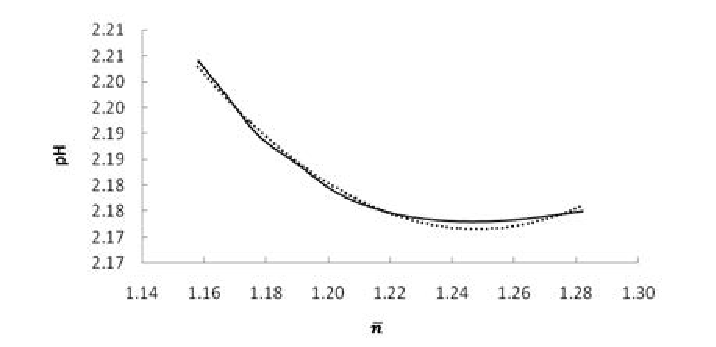
\includegraphics{figures/oxalic-acid-n-geq-1.15.pdf}
  \caption{这是手册中的 ``乙二酸$\overline{n}\geq 1.15$数据段曲线及其拟合曲线 (实线--实际曲线, 虚线--拟合曲线)", 图片模糊字体不对, 是反面例子.}\label{fig:xlccd-single}
\end{figure}

\begin{figure}[htbp]
  \centering
  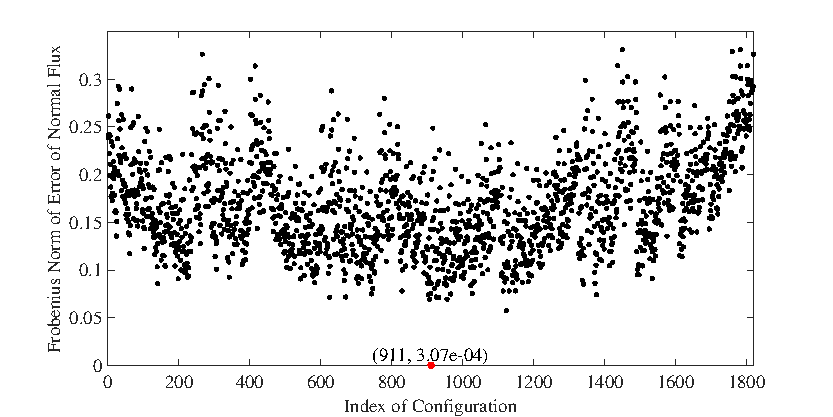
\includegraphics{figures/source-block-find-position.pdf}
  \caption{源方块位置寻找散点图. 横轴为四个源方块的所有可能出现的位置组合, 共 1820 种情况, 按照字典序 (MATLAB 中 nchoosek 函数的输出顺序) 排列. 纵轴为这种位置组合下法向通量与条件中法向通量误差的 Frobenius 范数. 结果发现第 911 种组合, 即组合$(3, 5, 8, 15)$对应的误差显著小于其它组合, 这种组合的误差仅约为 $3.07\times 10^{-4}$, 因此认为这种组合即为所求.}\label{fig:sb-fp}
\end{figure}

\begin{figure}[htbp]
  \centering
  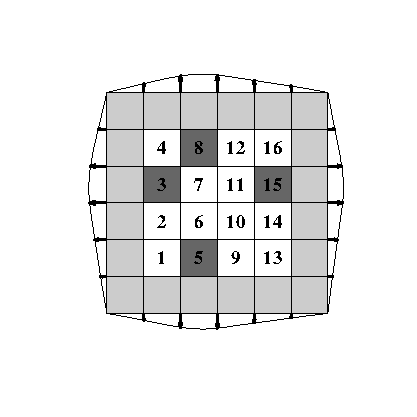
\includegraphics{figures/source-block-picture.pdf}
  \caption{源方块位置示意图. 浅灰色方块表示源方块不可能出现的位置, 白色方块表示源方块可能出现但没有出现的位置, 深灰色方块 $(3, 5, 8, 15)$ 表示源方块最终出现的位置. 最外侧的箭头与曲线示意该位置该方向法向通量的大小, 箭头长度越长法向通量越大.}\label{fig:sb-pic}
\end{figure}

在排版过程中我们会遇到多列子图的情况, 我们在文档类中已经引用了 \pckg{subcaption} 宏包, 并做好了子图的图序和图题的格式定制. 我们利用 \verb|subfigure| 环境来排版子图, 它的第一个可选参数 \verb|<outer-pos>| 表示子图整个盒子的垂直位置, 可选项为 ``c", ``t", ``b", ``T", ``B", 可以参考 \pckg{latex2e} 文档中关于 \verb|minipage| 环境及参数的介绍以及 \pckg{subcaption} 宏包文档的相关内容来明白这些参数以及其它可选参数的含义. \verb|subfigure| 环境的必选参数表示这张子图及图题所占的宽度, 它不会帮你缩放插图, 但会决定图题所占的宽度, 注意一行之中所有子图的宽度之和不要超过 \verb|\textwidth|. 下面的例子中要注意仅在子图要换行的时候添加空行, 并确保每一行子图的图题要具有相同的行数, 还要注意 \verb|\hfil| 宏保证了这些子图之间以及与页边的水平间距合适, 关于 \verb|\hfil| 宏可以参考\href{https://tex.stackexchange.com/a/528921/184559}{这个回答}. 每张子图可以分别加上标签, 比如\ref{fig:tju}是我们多行多列子图的示例, 而\ref{fig:tjusub1}是其中第一张子图. 关于引用时标签输出格式的设定, 我们准备放到以后再研究.

\begin{figure}[htbp]
  \hfil
  \begin{subfigure}[b]{0.4\textwidth}
    \centering
    
\includegraphics{tongji-name-bacholar.jpg}
    \caption{同济大学图标 同济大学图标 同济大学图标 同济大学图标 同济大学图标}\label{fig:tjusub1}
  \end{subfigure}
  \hfil
  \begin{subfigure}[b]{0.4\textwidth}
    \centering
    
\includegraphics{tongji-name-bacholar.jpg}
    \caption{同济大学图标\\~}
  \end{subfigure}
  \hfil

  \hfil
  \begin{subfigure}[b]{0.4\textwidth}
    \centering
    
\includegraphics{tongji-name-bacholar.jpg}
    \caption{同济大学图标\\~}
  \end{subfigure}
  \hfil
  \begin{subfigure}[b]{0.4\textwidth}
    \centering
    
\includegraphics{tongji-name-bacholar.jpg}
    \caption{同济大学图标 同济大学图标 同济大学图标 同济大学图标 同济大学图标}
  \end{subfigure}
  \hfil
  \caption{同济大学图标}\label{fig:tju}
\end{figure}

\zhlipsum[1]

\subsection{表格}

我们先来整理一下手册对插图的要求. 手册第十九页的撰写规范中提到:
\begin{quote}
  每个表格应有表序和表题, 表序和表题应写在表格上方正中, 表序后空一格书写表题. 表序, 表题采用宋体小5号. 表格允许下页接写, 表题可省略, 表头应重复写, 并在右上方注明 {``\songti\upshape 续表 XX"}. 表格上下均应空一行.
\end{quote}
手册第五十一页及第五十二页的参考例文中提到:
\begin{quote}
  图表可横版.

  表格上下与正文之间各空一行;
  采用三线表, 两端与页面对齐;
  表中文字: 小五, 宋体 (英文 Times New Roman), 行距 18 磅, 段前 0 行, 段后 0 行.

  表序写在表题左方不加标点, 空一格写表题, 表题末尾不加标点, 表格逐章编序, 表序必须连续, 如表 4.4 表示第四章的第四个表. 表题: 小五, 宋体 (英文 Times New Roman), 居中置于表上方, 行距 18 磅, 段前 0 行, 段后 0 行.

  若表格分页, 则该表第 2 页的表题省略, 但表头应重写, 并在表右上方加注 ``续表 X.X";
  ``续表 X.X" 的格式: 小五, 宋体 (英文 Times New Roman), 行距 18 磅, 段前 0 行, 段后 0 行, 右空 2 格.
\end{quote}

现在我们应该来说一下应该如何排版表格. 类似于插图的情况, 我们做好了表序表题的格式定制, 设置好了 \verb|table| 环境的计数器. 我们利用 \verb|\captionsetup| 宏配置了 \verb|table| 环境的 \verb|position| 选项. 文档类中还引用了 \pckg{array} 宏包和 \pckg{booktabs} 宏包, 用来改良 \verb|tabular| 环境并制作漂亮的三线表.

类似于插图, 正文中的表格一般也以浮动体的形式出现. 绘制表格的方法, 其中参数的含义以及浮动体的介绍可以参考 \pckg{latex2e} 的文档, 我们就不在这里详细展开了. 需要注意的是 \verb|\caption| 宏应该写在 \verb|\includegraphics| 宏的上方, 同样如果需要用 \verb|\label| 宏则应放在 \verb|\caption| 宏之后. 还需要注意的是表格内各类元素的字体需要统一, 比如不能有的数字用数学字体, 有的数字用文字字体. \emph{在排版过程中我们发现手册第 50 页的参考例文中的表格, 似乎其上方的正文空了两行.} 我们并不准备对此进行模仿.

手册要求表格的两端与页面对齐, 关于这个排版需求我知道两种方法, 可以参考\href{https://tex.stackexchange.com/questions/10535}{这个问题}中的\href{https://tex.stackexchange.com/a/56552}{这个回答}和\href{https://tex.stackexchange.com/a/10540}{这个回答}. 两种方法的主要区别在于, 第一种方法没有改变每一列的宽度, 而是通过增加列之间的距离来实现表格宽度的增加, 不过第一列与最后一列离表格的边缘会比较近, 第一种方法不需要引用额外的宏包. 第二种方法通过增加每一列的宽度来实现表格宽度的增加, 需要引用 \pckg{tabularx} 宏包. 我们并没有在文档类中引用 \pckg{tabularx} 宏包, 用户若有需要可以自行引用. 文档类中为了设置表格中文字的格式在 \verb|tabular*| 环境和 \verb|tabularx| 环境之前添加了设置字体大小和行距的命令. \ref{tab:xlccd}展示了如何用第一种方法进行不跨页表格的排版. 之后我们还会考虑使用 \pckg{pgfplotstable} 宏包进行表格的排版, 因为那样可以省去我们在表格的每一个位置都加上数学环境的麻烦.

\begin{table}[htbp]
  \caption{草酸的部分数据列表}\label{tab:xlccd}
  \begin{tabular*}{\textwidth}{c @{\extracolsep{\fill}} cccc}
    \toprule
    $V\!\unit{mL}$ & $E\unit{mV}$ & $\mathrm{pH}$ & $[\hydrgenn]\unit{mod\cdot L^{-1}}$ & $\overline{n}$\\
    \midrule
    $\dotsb$ & $\dotsb$ & $\dotsb$ & $\dotsb$ & $\dotsb$\\
    \\
    $1.00$ & $2.62\times 10^2$ & $2.22$ & $6.07\times 10^{-3}$ & $1.14$\\
    $1.50$ & $2.60\times 10^2$ & $2.27$ & $5.42\times 10^{-3}$ & $1.10$\\
    \\
    $\dotsb$ & $\dotsb$ & $\dotsb$ & $\dotsb$ & $\dotsb$\\
    \bottomrule
  \end{tabular*}
\end{table}

非浮动体表格以及跨页表格的排版我们使用 \pckg{longtable} 宏包来实现. 只用 \pckg{longtable} 的话代码会有些复杂, 建议读者再引用 \pckg{pgfplotstable} 包, 文档类基于此提供了一个排版这类表格的简易接口:
\begin{verbatim}
  \typesetlongtable[<options>]{<caption>}{<label>}{<filename>}
\end{verbatim}
其中 \verb|<filename>| 是一个文本格式的数据文件, 目前的设置为第一行代表表头, 各列数据以逗号分隔, 各行数据以换行符分隔, 而我们希望用户可以通过 \verb|<options>| 来设置表头, 数据的形式 (字符或数学) 等宏包中提供的选项. \ref{tab:data-table} 是一个跨页表格的例子. 目前如果用户对我们提供的接口不满意, 可以参照文档类的源码自己定义相似的命令来使用 \pckg{pgfplotstable} 来达到排版要求, 也可以将就着直接使用 longtable 环境. 我们将要测试并改善这个接口.

\emph{要注意手册的示例中``{\songti 续表 XX}" 的中英文及阿拉伯数字均为宋体, 与示例旁边的叙述 (英文 Times New Roman) 矛盾了, 因此我们没有模仿这一行为.}

\subsection{代码}

手册对论文中所附代码块的排版没有具体要求, 不过一般代码块应该在附录中使用, 除非很有必要的情况不推荐在正文中放入代码块. 文档类中代码块采用 1.3 倍行距, 中文为仿宋字体, 中文的斜体采用楷体, 字号均为小五; 英文为 Courier New 字体, 字体大小经过缩放使得小写字母的高度与小五的 Times New Roman 字体的小写字母的高度相匹配. 代码块由 0.4pt 粗的边框包围, 代码块的标题与表题排版相同, 放在代码块上方, 字号小五, 行距 18bp.

一般来说代码高亮可以采用 \pckg{listing} 包或者 \pckg{minted} 包, 在文档类中这两个包都没有引用, 用户可以选用自己习惯的方式. 在这里推荐使用 \pckg{minted} 包, 文档类中也对此进行了配置并给出了接口, 使得大部分情况下用户不需要做额外配置就可以基本满足排版要求.

使用 \pckg{minted} 包进行代码高亮需要首先安装 \href{https://wiki.python.org/moin/BeginnersGuide/Download}{Python}, 以及 Python 中的 \href{https://pygments.org/download/}{Pygments} 包, 并在 {\LaTeX} 编译时添加 \verb|--shell-escape| 选项以启用外部程序.

代码块外部的边框是由 \pckg{tcolorbox} 宏包得到的, 目前还存在一些问题, 主要是代码块前后可能会产生 ``Underfull vbox" 的警告, 并且有不必要的竖直间距. 代码的文件路径中不要出现下划线, 这涉及到一些奇怪的字符问题.

排版代码块的方式如下:
\begin{verbatim}
  \usepackage{minted}
  \begin{listing}
    \caption{<caption>}\label{<label>}
    \tcbinputminted{<language>}{<filename>}
  \end{listing}
\end{verbatim}
跨页代码块也可以如此排版. 可以进行高亮的语言可以通过在命令行中输入
\begin{verbatim}
  pygmentize -L lexers
\end{verbatim}
进行查询. 因为大部分同学的环境中并不满足所需的依赖, 所以这个示例中就不展示用 \pckg{minted} 排版的效果了. 如果有安装完 Pygments 的同学想看示例, 可以将 tjuthesis.tex 中的
\begin{verbatim}
  \usepackage{minted}
\end{verbatim}
结束注释,
% \ref{code:JD-iter} 是一个较短 Matlab 代码块的例子, 而 \ref{code:NN-init} 是一个较长 Python 代码块的例子, 放入附录中.

目前我们提供了完全相同的 listing 环境和 longlisting 环境, 它们都不是浮动体, 将来我们会把 listing 环境设置为浮动体, 把 longlisting 环境设置为可以换页的环境.

要注意因为通常代码块中会含有大量的字符, 使用 MikTeX 发行版的用户可能会得到 TeX 容量超出限制的报错, 此时需要先查看 log 找到是哪些容量不够了, 然后按照\href{https://tex.stackexchange.com/a/548335/}{这个回答}中的方法来扩充可用容量. 如果代码块里有过长的行可能无法排版, 建议不要出现超过 80 个字符的行. 如果用户还遇到了其它错误, 可以先考虑删除所有的临时文件以及 \pckg{minted} 生成的缓存文件夹 (以 ``\_minted" 打头) 再重新进行编译.

% 如果代码块占用了接近一页的篇幅, 则很有可能会出现 ``Underfull \\vbox" 的信息, 因为此时会比较容易出现一页中有不到一行的竖直空白的情况, (我猜) {\LaTeX} 并不知道对此应该如何处理.

\subsection{算法}

前文说过在正文中放上代码块一般不是一个好的选择, 我们可以采用算法块的形式来概括代码, 设计良好的算法块可以使读者能轻松地跟上作者的思路.

手册对论文中算法块的排版没有具体要求. 文档类中算法块采用 18 磅行距, 字体与正文相同, 字号为小五. 算法块的边框与代码块相同, 均为 0.4pt 粗. 算法块的标题与表题和代码块标题排版相同, 放在算法块上方, 字号小五, 行距 18bp.

关于算法排版的宏包可以参考\href{https://tex.stackexchange.com/a/230789/}{这个回答}和\href{https://tex.stackexchange.com/a/594570/}{这个回答}, 我们也在这里概括一下其中的内容.
\begin{enumerate}
  \item \pckg{algorithm} 宏包提供了代码块的浮动体外壳 (wrapper), 即提供了一个类似于 figure 和 table 的环境, 文档类中采用了别的方式实现了这个宏包的效果, 请不要引用这个宏包.
  \item \pckg{algorithmic} 宏包提供了具体排版代码的环境 algorithmic, 目前已经有替代的宏包了.
  \item \pckg{algorithmicx} 宏包是 \pckg{algorithmic} 宏包的替代, 也提供了具体排版代码的环境 algorithmic, 并且提供了接口允许用户做一定的配置.
  \item \pckg{algpseudocode} 宏包是 \pckg{algorithmicx} 宏包的一种样式, 模仿了 \pckg{algorithmic} 的样式和接口, 它会引用 \pckg{algorithmicx} 宏包, 因此只需要引用 \pckg{algorithmicx} 宏包即可.
  \item \pckg{algorithm2e} 宏包提供了另一种具体排版代码的环境, 提供的接口有一定的区别.
  \item \pckg{algpseudocodex} 宏包是一种新的宏包, 试图统一上述宏包. 我还没有了解过这个宏包, 有兴趣的读者可以自行查阅一下它的文档.
\end{enumerate}

文档类中针对 \pckg{algorithmicx} 宏包做了配置, 并保持了宏包所给出的接口, 使用方法为:
\begin{verbatim}
  \usepackage{algpseudocode}
  \begin{algorithm}[htbp]
    \caption{<caption>}\label{<label>}
    \begin{algorithmic}
      <content>
    \end{algorithmic}
  \end{algorithm}
\end{verbatim}
用户也可以选用其它方式, 只不过可能需要自行调整样式以使得格式统一. \ref{alg:twolevel} 是一个算法块的例子.

\begin{algorithm}[htbp]
	\caption{两水平加性Schwarz预条件处理的Jacobi-Davidson迭代法}\label{alg:twolevel}
	\begin{algorithmic}
    \Require{$u^{1}$, $\varepsilon$}
    \Comment{初值和终止准则}
	  \State{$\lambda^{1} = \Rq(u^{1})$, $W^{1} = \mspan \{u^{1}\}$}
    % 设$\lambda^{1}_h \leq \lambda^{1} \leq \lambda^{1}_H$.
	  \While{$\vert \lambda^{k+1}-\lambda^{k}\vert \geq \varepsilon$}
      \State{$t^{k+1}=\textup{CorrectionEquationSolver}(u^k)\in\mspan \{u^{k}\}^{\perp}$}
      \Comment{利用校正方程求解$t^{k+1}$}
      \State{$W^{k+1} = \mspan \{ W^{k},t^{k+1}\}$}
      \Comment{扩展搜索空间}
      \State{$u^{k+1} = \argmin_{\norm{u^{k+1}}=1} \Rq(v), v\in W^{k+1}$}
      \Comment{更新$u^{k+1}$}
      \State{$\lambda^{k+1} = \Rq(u^{k+1})$}
      \State{$k \gets k+1$}
	  \EndWhile
	\end{algorithmic}
\end{algorithm}

\zhlipsum[1]

\subsection{文献引用}\label{sec:exm-bib}

采用 \verb|\upcite| 宏和 \verb|\parencite| 宏来引用文献, 具体效果见 \ref{tab:cite-cmd}. \verb|\cite| 宏被定义为
\begin{verbatim}
  \let\cite\upcite
\end{verbatim}
即与 \verb|\upcite| 宏相同.

对于数学与应用数学专业的同学, 文献引用可以采用数学常用的格式. 目前来说仍应该按照引用顺序编号, 引用时不需要上标, 外文文献的作者名字也不用按照国标示例全大写. 如果一本图书只引用同一处内容, 则可以在参考文献表中标注页码; 如果图书广泛引用, 则不需要多次重复著录和标注页码. 我们也定义了 \verb|\thmcite| 宏来引用文献中的定理. 为了参考文献示例的需要, 我们来多搞点文献, 使得一共有十个及以上的文献 \cite{atiyah_introduction_1969, herrlich_axiom_2006, jacobson_basic_1985, jacobson_basic_1989, zariski_commutative_1958, zariski_commutative_1960, ciarlet_linear_2013, flaherty_riemannian_1992, munkres_topology_2000, ahlfors_complex_1978, milne_algebraic_2017}.

\begin{table}[htbp]
  \caption{文献引用常用命令示例}\label{tab:cite-cmd}
  \begin{tabular*}{\textwidth}{l @{\extracolsep{\fill}} ll}
    \toprule
    命令 & 效果\\
    \midrule
    \verb|\upcite{atiyah_introduction_1969}| & \upcite{atiyah_introduction_1969}\\
    \verb|\parencite{atiyah_introduction_1969}| & \parencite{atiyah_introduction_1969}\\
    \verb|\thmcite[Theorem 1.5.9]{riehl_category_2017}| & \thmcite[Theorem 1.5.9]{riehl_category_2017}\\
    \verb|\thmcites[Theorem 11.3]{altman_term_2017}| & \thmcites[Theorem 11.3]{altman_term_2017}[Proposition 3.1]{atiyah_introduction_1969}\\
    \verb|  [Proposition 3.1]{atiyah_introduction_1969}| & ~\\
    \bottomrule
  \end{tabular*}
\end{table}

测试一下翻译成外文的外文文献的著录 \cite{sally_history_1985}. 不太正式的参考资料\footfullcite{andrew_how_2016}我们在脚注里引用, 并且不著录进参考文献表中. 目前这个引用的著录格式与参考文献表中要求的格式不太相同, 不过短时间没有解决这个问题的动力.
